\documentclass[11pt,letterpaper]{article}
\usepackage[T1]{fontenc}
\usepackage{lmodern,amsmath,amssymb,booktabs,array,graphicx,xcolor,microtype}
\usepackage[margin=.84in,top=.80in,bottom=.78in,headheight=14pt]{geometry}
\usepackage{fancyhdr,enumitem}
\usepackage[colorlinks=true,urlcolor=teal!70!black,linkcolor=teal!70!black]{hyperref}
\definecolor{ink}{HTML}{193740}
\definecolor{teal}{HTML}{236D65}
\pagestyle{fancy}\fancyhf{}
\fancyhead[L]{\small\color{ink}Shortest surface paths on the oloid}
\fancyhead[R]{\small\color{ink}Unit-radius disks}
\fancyfoot[C]{\small\thepage}\renewcommand{\headrulewidth}{.3pt}
\newcommand{\heading}[1]{\section*{\color{ink}#1}}
\newcommand{\para}[1]{\smallskip\noindent\textcolor{teal}{\textbf{#1}}\enspace}
\newcommand{\len}{\mathop{\rm len}}
\newcommand{\RR}{\mathbb R}
\newcommand{\norm}[1]{\lVert #1\rVert}
\newcommand{\rt}{\sqrt{3}}
\newcommand{\dd}{\mathop{}\!d}
\setlength{\parindent}{1.1em}
\setlength{\parskip}{2pt}
\setlist{leftmargin=1.6em,nosep}
\hypersetup{pdftitle={Shortest surface paths on the oloid},pdfsubject={Ten points and 45 certified intrinsic distances}}
\begin{document}
\thispagestyle{plain}
{\color{teal}\sffamily\small INTRINSIC GEOMETRY}\par\vspace{5pt}
{\color{ink}\fontsize{28}{32}\selectfont\bfseries Shortest surface paths on the oloid}\par\vspace{6pt}
{\large Ten interior points, forty-five certified distances}\par\medskip
\noindent Two unit disks have centers $(-1/2,0,0)$ and $(1/2,0,0)$ in the planes $z=0$ and $y=0$, respectively. The surface $S$ is the boundary of their convex hull. The ten points below lie on different straight rulings, strictly between the two circular edges. They occupy all four sign combinations of $y,z$. For one pair the shortest route crosses both circular edges, and for another the two choices of crossing are separated by less than seven millionths of the disk radius.

\para{Exact coordinates.} In each row put $c=(1-h^2)/(1+h^2)$ and $k=2h/(1+h^2)$. Take the indicated fraction $s$ of the way from $A$ to $B$, then apply the signs in the fourth column to its transverse coordinates.
\[
 A=(-\tfrac12-c,k,0),\qquad
 B=(\tfrac12-c/(1+c),0,\sqrt{1+2c}/(1+c)).
 \tag{1}
\]
The last three columns give the signed spatial coordinates rounded to six decimals.
\begin{center}\small
\renewcommand{\arraystretch}{1.13}
\begin{tabular}{@{}ccccrrr@{}}\toprule
 Point & $h$ & $s$ & $(\varepsilon_y,\varepsilon_z)$ & $x$ & $y$ & $z$\\\midrule
\csname @@input\endcsname data/point_rows.tex 
\bottomrule\end{tabular}
\end{center}
\begin{center}
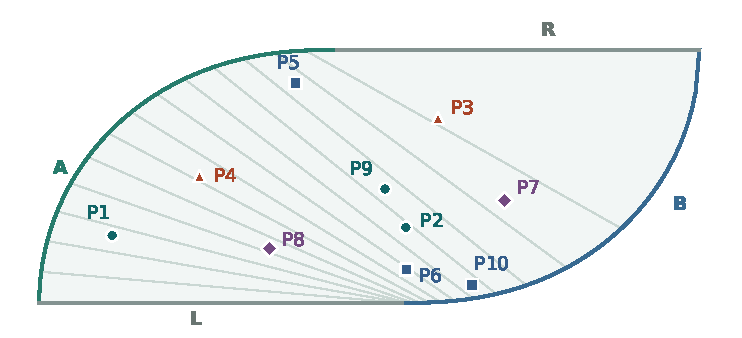
\includegraphics[width=.83\linewidth]{figures/chamber.pdf}
\end{center}
{\small\noindent Each point is shown after folding the signs and flattening one quarter of $S$. Pale lines are rulings. The labels A and B mark circular edges in space. L and R mark straight rulings in the symmetry planes. The drawing places the planar coordinate $V$ horizontally and $U$ vertically.}

\newpage
\heading{The 45 shortest lengths}
A row entry $(i,j)$ gives the distance from $P_i$ to $P_j$ in units of the disk radius. Each printed value is correctly rounded to eight decimal places. Read each route in order from the smaller index to the larger. A dash is a straight segment in one developed patch. Reverse the letters to trace the path back.
\begin{center}\small
\renewcommand{\arraystretch}{1.13}
\setlength{\tabcolsep}{4pt}
\begin{tabular}{@{}crl@{\hspace{1.55em}}crl@{\hspace{1.55em}}crl@{}}\toprule
 Pair& Length& Via&Pair& Length& Via&Pair& Length& Via\\\midrule
\csname @@input\endcsname data/distance_rows.tex 
\bottomrule\end{tabular}
\end{center}

\para{What the route tells you.} A and R each change the sign of $z$. A is a circular edge of the disk in $z=0$, and R is the straight ruling in that plane. B and L each change the sign of $y$. B is a circular edge of the disk in $y=0$, and L is the straight ruling in that plane. The eight direct, twenty-five single-crossing and twelve double-crossing entries give globally shortest routes on the entire closed surface.

\para{A route crossing both circular edges.} Starting at $P_4$ in $(+,-)$, cross A into $(+,+)$, then B into $(-,+)$ and continue to $P_{10}$. Its three legs have approximate lengths $0.546383$, $1.608380$ and $0.083799$. The exact distance lies in
\[
 [\,2.23856238329356,\;2.23856238339352\,].
\]
Every other reduced crossing pattern is at least $2.30821106873358$ long. Both contacts are interior to their respective exposed arcs. Their approximate spatial coordinates are $(-0.52823,0.99960,0)$ and $(0.27161,0,0.97357)$. The ambient chord from $P_4$ to $P_{10}$ has length $1.74218$ and passes inside the solid.
{\centering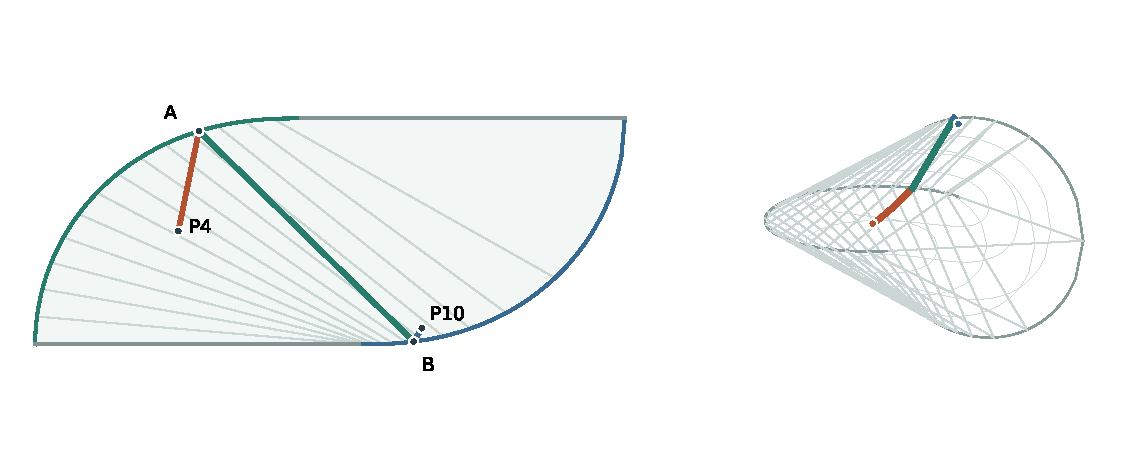
\includegraphics[width=.79\linewidth]{figures/two_creases.pdf}\par}
{\small\noindent Left, the three legs folded into one planar patch. Right, the same path lifted to the transparent surface. The last leg is short because $P_{10}$ lies close to the second circular edge.}

\newpage
\heading{The four pieces of the surface}
Write $D_A,D_B$ for the filled disks and $K=\operatorname{conv}(D_A\cup D_B)$. Every point of $K$ is an interpolation between one point in each disk, by grouping the coefficients in a convex combination. The signed reflections in $y$ and $z$ preserve $K$ and its boundary. We first work in the closed quarter $C=S\cap\{y,z\ge0\}$, using the coordinates of the supplied archive \cite{archive}.

Let $0\le t\le T=2\pi/3$, with $c=\cos t$, $k=\sin t$. Thus $h=\tan(t/2)$ in (1). Define $A(t),B(t)$ by (1) and
\[
 X(s,t)=(1-s)A(t)+sB(t),\qquad 0\le s\le1.
\]
The vector $n=(-c,k,\sqrt{1+2c})$ has projected lengths $1$ on the first disk plane and $1+c$ on the second. Its two disk support heights coincide:
\[
 n\cdot A=c/2+1=n\cdot B.
\]
Each disk meets its supporting plane in just its indicated point. The entire segment $AB$ therefore belongs to $C$.

Conversely, take $p\in C$ with $y,z>0$. At a supporting plane through $p$, a representation of $p$ as a disk interpolation uses both disks with positive weights, hence both disks must attain the common support height. Neither planar projection of the supporting normal is zero. A normal perpendicular to one disk would strictly favor the other. Normalize the first projection to length one and denote it by $(-c,k)$. The single disk maximizers and $y,z>0$ imply $k>0$ and $n_z>0$. Equality of support heights forces the other projected length to be $1+c$, giving $n_z^2=1+2c$. Hence $p=X(s,t)$ with the two endpoints in (1). Points on the coordinate planes follow by closure. For detail, the origin lies inside $K$ (it contains the six points $\pm e_i/2$). Radial projection from this origin identifies $S$ with the unit sphere, so directions with $y,z>0$ approximate every point of the closed quarter. The parametrized image is compact.

The parametrization is one-to-one. A point with positive weights in a second ruling representation forces both new endpoints to maximize the original supporting functional. Those maximizers are unique. A point at a circular endpoint cannot also have a positive-weight representation: using its own supporting functional would give the original two distinct disk endpoints and hence a strict interior point of their segment. Within either exposed arc the parameter is injective. The arcs are disjoint: a shared point would lie on the $x$-axis, whereas the only axis point of each exposed arc is its own outer tip. Compactness now gives a homeomorphism from the closed rectangle onto $C$. In particular its four sides account for all places a sign can change.

\para{The two straight sides.} At $t=0$ the whole ruling lies in $y=0$ (L), and at $t=T$ it lies in $z=0$ (R). At $s=0$ the exposed circular arc is in $z=0$ (A), and at $s=1$ the other arc is in $y=0$ (B). This identifies the exposed arcs of the two generating circles.
\begin{center}
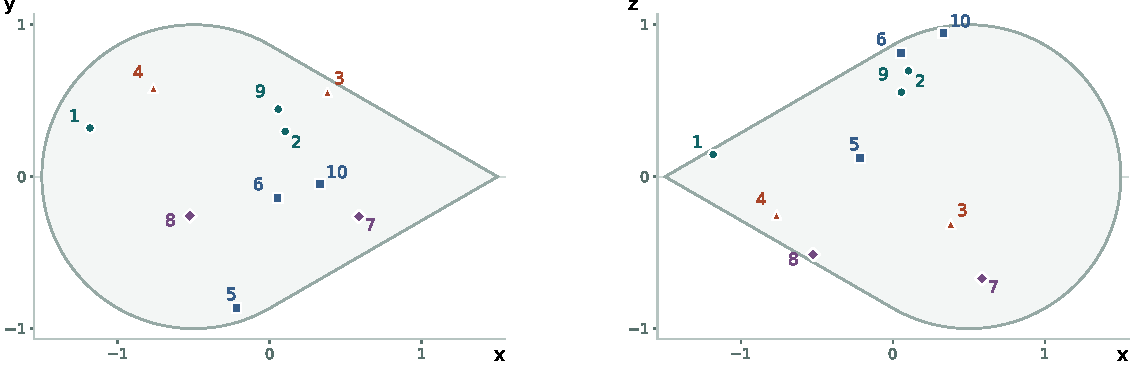
\includegraphics[width=.82\linewidth]{figures/projections.pdf}
\end{center}
{\small\noindent Orthogonal projections of the ten spatial points onto the $xy$-plane (left) and $xz$-plane (right). The outline in each view is the convex hull of a unit disk and the far tip of the other disk. Labels give the point indices.}

\newpage
\heading{Developing a quarter into the plane}
Use planar coordinates $(U,V)$ and write $a(c)$ for the image of $A(t)$. Put $c^*=-c/(1+c)$, $W=2\pi\rt/9$, $K_0=\rt(6+\log4)/9$, and $H=K_0+\rt$. The developed endpoints and ruling are
\begin{align}
 a_U(c)&=\frac{2\rt}{9}\left(\sqrt{2(1-c)(1+2c)}
              +\arccos\frac{\sqrt2\,c}{\sqrt{1+c}}\right),\nonumber\\
 a_V(c)&=\frac{\rt}{9}\left(4(1-c)+\log\frac2{1+c}\right),\nonumber\\
 b(c)&=(W,H)-a(c^*),\qquad F(s,t)=(1-s)a(c)+s b(c).
 \tag{2}
\end{align}
These are the elementary development formulas of Dirnböck and Stachel \cite{ds}, in coordinates matched to (1). Here is a verification of the metric, including a parameter that stays regular at the ends.

Set $v=\sin\theta=\tan(t/2)/\rt$, $w=\cos\theta$, $d=1+3v^2$, $0\le\theta\le\pi/2$, and $\beta=\operatorname{atan2}(2v,w)$. Then $c=(1-3v^2)/d$, $t'=2\rt w/d$ and $\beta'=2/d$, with primes denoting $\theta$ derivatives. In \emph{reversed} planar coordinates $(V,U)$ define $\phi=2(\theta-\beta)$, $e=(\cos\phi,\sin\phi)$ and $J(x,y)=(-y,x)$. One obtains
\[
 b-a=\rt e,\qquad
 \frac{\dd a}{\dd\theta}=t'(v e+w J e).
 \tag{3}
\]
To check these identities, (2) reads $a_V=\rt[\log d+8(1-1/d)]/9$ and $a_U=2\rt[\theta+\beta+6vw/d]/9$. Indeed $\theta+\beta\in[0,\pi]$ has the cosine in (2). For $c^*$ substitute $v^*=w/\sqrt d$, $w^*=2v/\sqrt d$, $d^*=4/d$. This gives $\theta^*=\pi/2-\beta$, $\beta^*=\pi/2-\theta$. Subtraction in (2) then yields
\[
 e=\left(\frac{1+v^2+2v^4}{d},\,\frac{-2v(1+v^2)w}{d}\right).
\]
Differentiating $a$ gives $\dd a/\dd t=(v(3+v^2),w^3)/d$ in the same reversed coordinates, which is $v e+wJe$. These formulas extend continuously to both ends.

In space let $E=(B-A)/\rt$. Squaring the coordinates in (1) gives $\norm{B-A}^2=3$. With $A_t=\dd A/\dd t$ we have $A_t\cdot E=v$ and $A_{tt}\cdot E=\rt w^2/2$ by substitution. In the open parameter interval $N=(A_t-vE)/w$ is a unit vector orthogonal to $E$. Since $A',B'$ are tangent to the common support plane, $E'$ is in that plane, and since $\norm E=1$, $E'=\lambda N$. Differentiating $A_t\cdot E=v$ gives
\[
 \lambda=\frac{w-t'\rt w^2/2}{w}=\frac{2(3v^2-1)}{d}=\phi'.
\]
Thus $X_s=\rt E$ and $X_\theta=t'(vE+wN)+s\rt\lambda N$. Equations (3) give the same coefficients for $F_s,F_\theta$ in the orthonormal frame $(e,Je)$. Equality of their Gram matrices proves that every tangent displacement has the same norm before and after development. The absolute Jacobian equals
\[
 \frac{6}{d}\big((1-s)w^2+2s v^2\big),
 \tag{4}
\]
which vanishes only at $(s,\theta)=(1,0),(0,\pi/2)$. In this parameter both maps are continuously differentiable up to the sides, as the displayed formulas show.

\newpage
\heading{Why every chord in the development lifts}
In the original order $(U,V)$, the tangent angle of the lower arc $a$ measured from $+U$ is $2\beta-\theta$. It increases from $0$ to $\pi/2$, since its derivative is $4/d-1\ge0$. Also $U$ strictly increases along the open arc. Thus $a$ is the graph of a convex function $f$ on $[0,W]$, with $f(0)=0$ and $f(W)=K_0$. The upper arc is the graph of the concave function $g(U)=H-f(W-U)$. Convexity bounds $f(U)$ by $K_0U/W$, and hence $g(U)-f(U)\ge\rt$. The region
\[
 D=\{(U,V):0\le U\le W,\quad f(U)\le V\le g(U)\}
\]
is compact and convex. At $U=0$ and $U=W$ its boundary sides are exactly L and R.

To show $F$ maps onto $D$ exactly once, fix $0<U<W$. Both $a_U$ and $b_U$ increase strictly with $\theta$ from $0$ to $W$ (use the formula with $c^*$ for $b$). In the open interval $b_U<a_U$ by the formula for $e$. Therefore the admissible parameters form the interval from $a_U^{-1}(U)$ to $b_U^{-1}(U)$, and $s=(a_U-U)/(a_U-b_U)$ is forced. On this interval the derivative of $V$ at fixed $U$ is $\det(F_s,F_\theta)/(F_s)_U>0$. Indeed the determinant in the order $(U,V)$ is minus (4), and $(F_s)_U<0$. The slice runs exactly once from $f(U)$ to $g(U)$. At $U=0,W$ the limiting ruling parametrizes its full side. Consequently $F$ is a homeomorphism onto $D$. Denote $F\circ X^{-1}:C\to D$ by $\Phi$.

\para{Lengths on the closed chamber.} For any continuous curve, length is the supremum of Euclidean chord sums over finite ordered partitions of its time interval, possibly $+\infty$. On a regular parameter neighborhood and for any $\eta>0$, corresponding chords under $X,F$ have length ratios between $(1+\eta)^{-1}$ and $1+\eta$ after the neighborhood is made small enough. To see this, approximate both differences by the differentials at its center, with error at most $\delta$ times the parameter displacement. This uses continuity of the derivatives and integration along a parameter segment inside a small convex rectangle. The two linearized norms agree, and are at least $m>0$ times the displacement by (4). Choose $\delta<m$ with $(m+\delta)/(m-\delta)\le1+\eta$. The same reasoning covers regular points on a side.

Partition any compact regular subarc finely enough to use these neighborhoods. Refining any chord partition and then letting $\eta$ tend to zero gives the developed endpoint displacement bound by the original length. Continuity gives the same result when a singular point occurs at either end only. For arbitrary subarcs, first subdivide time so that each piece can meet at most one of the two exceptional points, using uniform continuity and their positive separation. If a piece meets that point, split at its first and last visit. The two developed values there coincide, so the endpoint estimate follows from the two outside pieces and the triangle inequality. This also handles an infinite set of visits. Applying the estimate on every part of any partition gives $\len(\Phi\gamma)\le\len(\gamma)$. The identical argument for $\Phi^{-1}$ proves equality. In particular every chord in $D$ has a lift of exactly its Euclidean length, including chords ending on circular edges.

\newpage
\heading{The global minimum over all surface paths}
For any $p\in S$ put $\sigma(p)=(p_x,|p_y|,|p_z|)$ and $\bar p=\Phi(\sigma(p))$. The fold $\sigma$ preserves $S$ and contracts ambient distances by the ordinary absolute-value inequality. Given any continuous surface path $\gamma$ and any subinterval $[u,v]$, the preceding length equality therefore gives
\[
 \norm{\overline{\gamma(u)}-\overline{\gamma(v)}}\le
 \len\bigl(\gamma|_{[u,v]}\bigr).
 \tag{5}
\]
This inequality applies even when $\gamma$ switches sheets infinitely often.

For precise boundary point coordinates, write $a_T(f)=a(\cos(Tf))$ for $0\le f\le1$. The four gate parametrizations in the $(U,V)$ plane are
\[
 A_f=a_T(f),\quad B_f=(W,H)-a_T(f),\quad
 L_f=(0,\rt f),\quad R_f=(W,K_0+\rt f).
 \tag{6}
\]
Here A and B each use their own circle's arc length divided by $T$. For a word $w=g_1\cdots g_k$ let
\[
 M_w(p,q)=\min_{0\le f_1,\ldots,f_k\le1}
       \sum_{j=0}^{k}\norm{z_{j+1}-z_j},\qquad
 z_0=\bar p,\quad z_j=(g_j)_{f_j},\quad z_{k+1}=\bar q .
 \tag{7}
\]
The empty word gives just $\norm{\bar q-\bar p}$. Each minimum exists by continuity on a compact cube.

\para{Distance theorem.} For endpoints with nonzero transverse coordinates, the exact surface distance is the minimum of (7) over the following words. The formula applies in particular to every pair in the table.
\begin{center}\small
\begin{tabular}{@{}ll@{}}\toprule
Signs that differ & Admissible words\\\midrule
Neither & Empty word\\
$y$ alone & B, L\\
$z$ alone & A, R\\
Both & BA, BR, LA, LR, AB, AL, RB, RL\\\bottomrule
\end{tabular}
\end{center}
For the lower bound, each differing coordinate must vanish at some time by continuity. Select one such time per coordinate and sort them. A zero of $y$ places the folded path on B or L, and a zero of $z$ places it on A or R. Apply (5) to the resulting at most three subarcs and sum. Simultaneous zeros give a middle segment of length zero. The argument requires no upper bound on how often a path crosses either plane.

For attainment, connect a minimizing tuple in (7) by straight segments in $D$. Lift them by $\Phi^{-1}$ and reflect each leg into the current sign quadrant. Switch its indicated sign at each gate. The adjacent endpoints in space coincide because the changed coordinate is zero there. This constructs a continuous path on $S$ of exactly the displayed sum and with the required endpoints. Taking the least admissible word gives the result. Curved seams require this minimization over their contact points. In particular, reflecting an entire planar patch in a tangent to a curved seam would in general give an incorrect distance.

\newpage
\heading{Exact formulas and checked decimal bounds}
For each table entry, insert its listed word into (7) to obtain an exact expression requiring at most two real parameters. Twenty-five entries also have elementary formulas with no minimization. Set $J_L(U,V)=(-U,V)$ and $J_R(U,V)=(2W-U,V)$. Whenever the winning word uses only L and R, including the empty word, one has
\[
 d(P_i,P_j)=\norm{\bar P_i-J_{g_1}\circ\cdots\circ J_{g_k}(\bar P_j)}.
 \tag{8}
\]
Reflection straightens a broken line through a straight side. Conversely the chord to the reflected target is feasible when it meets the indicated \emph{finite} sides in order. For our entries this is verified by intersecting each vertical copy $U=u$ with the chord from $p$ to its unfolded endpoint $q'$. The intersection height is $p_V+(q'_V-p_V)(u-p_U)/(q'_U-p_U)$. The included \texttt{straight\_routes.py} checks the parameters and strict height inequalities with rational intervals. For example $P_2\to P_8$ uses RL and $q'=\bar P_8+(2W,0)$.

\para{How the remaining minima are certified.} We enclose the exact elementary coordinates at dyadic parameter values in rational boxes. A feasible tuple gives an upper bound using the lengths between box centers plus their endpoint errors. A lower bound must hold throughout each parameter cell, including where the optimizer did not sample. For a gate $G$ on $[l,r]$, its image lies within $M(r-l)^2/8$ of its endpoint chord if $\norm{G''}\le M$. This follows by integrating the second derivative against the linear-interpolation error kernel, whose absolute integral at $x$ is $(x-l)(r-x)/2$. From the turning angle $2\beta-\theta$ and $t'=2\rt w/d$, the absolute curvature in arc length is $\rt w/2$. Both circular gates thus have $M\le T^2<5$ in normalized parameter, including endpoints by limits. For L and R take $M=0$.

Enlarge that chord tube by the larger of its two endpoint box radii. Let the resulting segment and radius at stop $j$ be $[a_j,b_j]$ and $r_j$, allowing a point segment for each endpoint. Choose any vectors $d_j$ of norm at most one on the links. Cauchy--Schwarz bounds each link length below by its displacement dotted with $d_j$. On summing, the coefficient of stop $j$ is $v_j=d_{j-1}-d_j$, where the missing end directions are zero. A rigorous lower bound for the whole cell is therefore
\[
 \sum_j \left[\min(v_j\!\cdot a_j,v_j\!\cdot b_j)-r_j\norm{v_j}\right].
 \tag{9}
\]
This estimate works for both parameter orders, touching gates, and vanishing legs. Subdividing the longest parameter interval gives a binary tree whose leaves cover the whole cube. Each leaf supplies a bound of type (9). Tree coverage and the feasible upper path establish the complete interval for each pair.

\para{Crossing locations.} For $P_6\to P_9$, L wins. Its distance lies between $0.71145000013345$ and $0.71145000014262$. Every route via B has length at least $0.71145216156272$. The B endpoint $B_1$ gives an explicit feasible length below $0.711456882267$, so the gap between the two choices is less than $0.000006883$. For $P_4\to P_{10}$, restricting all possible minimizing AB contacts gives $f_A\in[0.7365,0.7366]$, $f_B\in[0.8600,0.8601]$. The additional tree covers the square by cells wholly inside the rectangle and cells whose lower bound exceeds the feasible upper bound. This proves both hits occur in the interiors of the circular edges.

\newpage
\heading{Reproduction and Lean formalization}
\para{Checking the numbers.} Run \texttt{python3 code/verify.py} from the extracted directory. It checks all 45 pairs and their 154 admissible words using the saved trees and integer arithmetic. There are 4{,}486 leaf bounds or containment checks including the separate two-contact check. The widest distance interval has width $9.996\times10^{-11}$, and both endpoints of every interval round to the same eight-place decimal. Each nonempty winning word is separated from all alternative words for that pair. The CSV records the bounds, a dyadic feasible contact tuple, and a lower bound for every alternative taken together. The dyadic tuple gives a near-minimizer. The global bounds determine the rounded distance.

The evaluator uses endpoints with denominator $10^{42}$ internally, rounded outwards at each operation, then exports boxes with denominator $10^{14}$. Square roots use integer floor-square brackets. Cosine and reduced arctangent use their Taylor polynomials with the first omitted term as error. The half-angle identity brings the arctangent arguments below $1/2$. Machin's identity gives $\pi$. For $\log x$, $1\le x\le4$, the positive series $2\sum y^{2k+1}/(2k+1)$ with $y=(x-1)/(x+1)$ has tail at most $2y^{2n+1}/((2n+1)(1-y^2))$ after $n$ terms. The independent floating-point script evaluates the chart through $\theta,\beta$, optimizes each admissible word, and agrees with all certified intervals.

\para{Lean targets.} \texttt{lean/SurfaceDistance.lean} defines both filled disks in $\operatorname{EuclideanSpace}(\RR,\mathrm{Fin}\;3)$, the frontier of their convex hull, continuous competitors on $[0,1]$, length as extended nonnegative variation, and intrinsic distance as the infimum of those lengths. It defines (1), (2), both sign-change sets, the ten points, the route infima, and the integer endpoints of the 45 intervals. It includes proof scripts for splitting variation, bounding by one or two ordered hits, and the infimum with an attaining curve. The two concrete goals are \texttt{ExactTable} and \texttt{NumericalTable}. The supplied Lean source is an uncompiled outline. A path to their kernel proofs is as follows.

\begin{enumerate}[itemsep=2pt]
\item Prove that the images of the spatial and planar rectangles are respectively $C,D$ and use compactness for both inverse maps. Prove (3)--(4) after the change to $\theta$. Formalize the regular chord comparison and finite exceptional-point argument to obtain equality of variations, then compose with the contracting absolute-value fold.
\item Use the intermediate value theorem for zero coordinates and the generic ordered-hit lemmas for the lower bound. Use compact minima, affine segments in the convex set $D$, and pasting reflected inverse lifts for attainment. Apply the infimum lemma to obtain \texttt{ExactTable}.
\item Prove interval-operation soundness, the two Taylor remainders, and (9) for bounded-norm integer directions. Define a recursive checker on the supplied trees, prove its soundness by induction on a tree, then evaluate it on the finite data to obtain \texttt{NumericalTable}. The detailed roadmap specifies the branch and leaf encodings and endpoint conventions.
\end{enumerate}

\small
\begin{thebibliography}{2}
\bibitem{ds} H. Dirnböck and H. Stachel, \emph{The Development of the Oloid}, Journal for Geometry and Graphics \textbf{1} (1997), 105--118, especially Theorems 1--3. \href{https://www.geometrie.tuwien.ac.at/stachel/jgg0113.pdf}{Author's copy}.
\bibitem{archive} \emph{The solid oloid in intuitionistic primitive recursive arithmetic}, supplied \texttt{oloid\_ipra.zip}, sections on the regular quarter and projected sweep. The geometric proof here uses ordinary real analysis in Lean's intended metatheory.
\end{thebibliography}
\end{document}
